\chapter*{Simulations of classical and pure exploration}
\label{cha:simulations} % (labels for cross referencing)

\section{Description}

Fortunately, all classical bandit algorithms mentioned in this paper are all relatively simple to implement, in that they all have closed-form solution. Given some inputs, they all perform some kind of elementary calculation and/or sampling, then return a result. The only exception is Ripple \ref{sec:ripple}, which requires K binary searches per iteration, which is not difficult to implement.



\section{Brief Implementation Notes}

In order to simulate both classical and pure exploration bandits, and to assess how easy it is to implement them, I attempted to program all in the Python programming language – Python is a very flexible language, and even though it’s not the fastest language out there, the same implementation methods can be used across other potentially more faster programming languages.

For the simulation data, I'm going to draw up data from our running examples, which will be as follows:

\begin{enumerate}
    \item \textbf{Substance Synthesis Example}
    \begin{itemize}
        \item Description: We're going to take a set of some resistors, most of which have very poor performance, but some have a much higher success rate. This test is particularly good for testing two factors at once: the regret used to effectively disregard the poor-performing arms and the regret used to decide which of the remaining arms is best.
        \item Specifics: We have 6 arms, each binomial with the probability of success being [0.1, 0.15, 0.2, 0.25, 0.85, 0.9]. The time-frame is over 1000 steps.
    \end{itemize}
    
    \item \textbf{Consumer Pricing Example}
    \begin{itemize}
        \item Description: We're going to simulate an animal shelter trying to encourage people to adopt. They have some indicators about what adverts are best (if the algorithm can use them), but otherwise don't have a defined strategy. Hence, they're opting to mass produce adverts hoping to find one that attracts their target market.
        \item Specifics: We have 20 arms, each binomial with the probability of success being [0.02, 0.03, 0.04, 0.05, 0.06, 0.02, 0.03, 0.04, 0.05, 0.06, 0.02, 0.03, 0.04, 0.05, 0.06, 0.02, 0.03, 0.04, 0.05, 0.09]. If usable, they have some prior data from a customer survey showing their favourite adverts (successes) - [1, 3, 3, 3, 3, 1, 3, 3, 2, 3, 2, 2, 3, 2, 2, 2, 2, 2, 3, 3]. The time-frame is over 100,000 steps, since online advertising can be executed on mass.
    \end{itemize}
\end{enumerate}



\section{Classical Bandit Algorithms}


\subsection{Randomized algorithm}

Firstly, I’m going to touch very briefly on the Randomized algorithm – since the performance is so incredibly poor across most scenarios, I’m not going to be showing any simulations of it since the graphs are unhelpful:

\begin{figure}[h!]
    \centering
    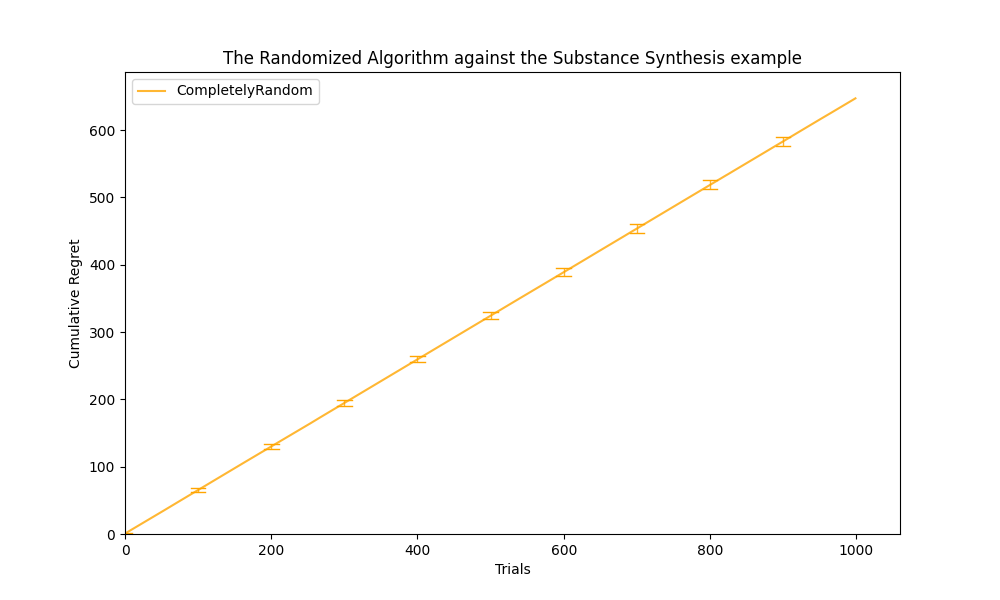
\includegraphics[width=17cm]{report/images/Randomized-Substance-Synthesis.png}
    \caption{The Randomised algorithm performs very poorly on all examples}
    \label{fig:stupid-random}
\end{figure}

\subsection{Epsilon-Greedy}

The Epsilon Greedy algorithm is very simple to implement, since it's only making an $\bigO{1}$ binary choice to perform either $\bigO{1}$ or $\bigO{K}$.

When comparing performance with variants of our epsilon function \epsilonFunction (which determines how likely we are to pick an arm at random), several problems become more obvious:

\subsubsection{Choosing the correct \epsilonFunction $\space$ is really hard}

Unfortunately, there's no universal solution to this problem, as the Epsilon Greedy algorithm only considers the current time-step as a parameter. Consequently, without prior knowledge of the number of arms involved, we risk either overexploring or underexploring the scenario.

For the plot in Figure \ref{fig:epsilon-degrade}, I'm using the geometric epsilon function, defined as $\epsilon(t) = \epsilon_0^t$. Unfortunately, since our example as "too few" arms for setting \contour{yellow}{$\epsilon = 0.98$}, it results in it exploring too much, accumulating too much regret.


\begin{figure}[h!]
    \centering
    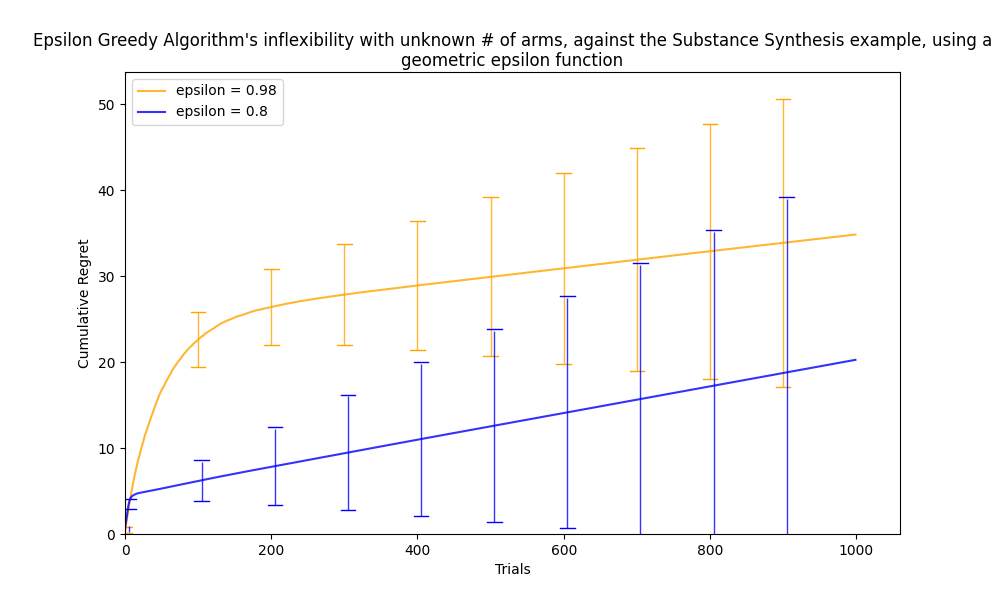
\includegraphics[width=17cm]{report/images/Epsilon-Greedy-SS-Poor-Degredation.png}
    \caption{It's difficult to pick the \epsilonFunction \space for the Epsilon Greedy algorithm in advance}
    \label{fig:epsilon-degrade}
\end{figure}

I chose the geometric epsilon function, purely because it has a high rate of exploration at the beginning, which decreases and doesn't get to insignificant probability of choosing at random. However, this choice was my personal guess, and it can be quite challenging to find a function that fits the scenario perfectly. Ideally, we'd have some prior knowledge of the data which determines which function to use. However, there's no built-in mechanism for this algorithm to incorporate prior knowledge, apart from guessing a suitable \epsilonFunction.

For example, a linear epsilon function with \contour{lightblue}{$\epsilon(t) = \epsilon_0 - t * 0.01$}, it appears to perform better on average when using the Substance Synthesis example in Figure \ref{fig:epsilon-linear}, but if we change the scenario to Consumer Pricing, it ends up performing worse in Figure \ref{fig:epsilon-linear-cp}

\begin{figure}[h!]
    \centering
    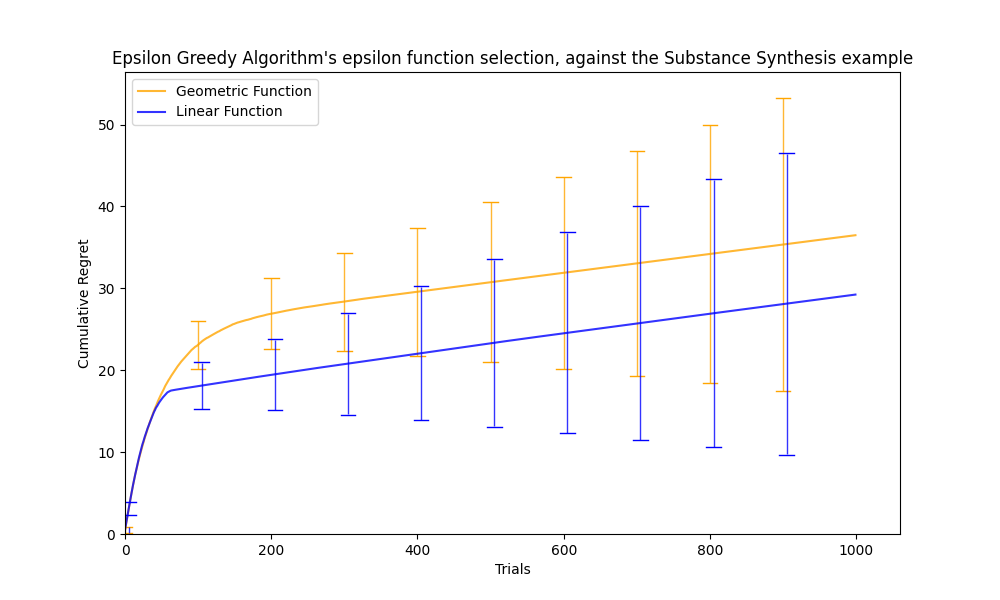
\includegraphics[width=17cm]{report/images/Epsilon-Greedy-Linear-Geometric.png}
    \caption{For this example, a linear \epsilonFunction \space appears to perform better}
    \label{fig:epsilon-linear}
\end{figure}

\begin{figure}[h!]
    \centering
    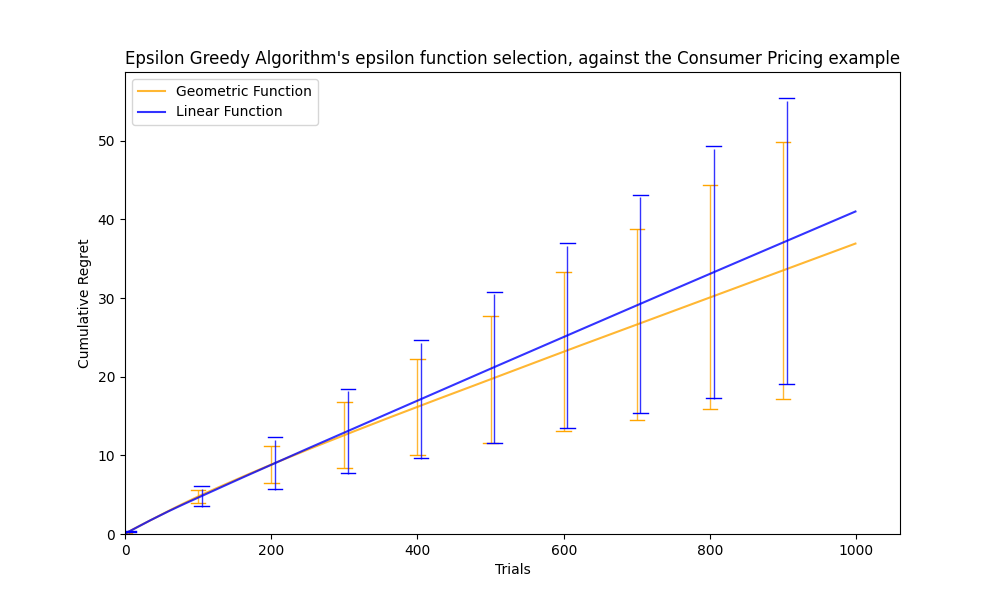
\includegraphics[width=17cm]{report/images/Epsilon-Greedy-Linear-Geometric-CP.png}
    \caption{However, tuning the epsilon function doesn't work when the scenario changes}
    \label{fig:epsilon-linear-cp}
\end{figure}


\subsection{Upper Confidence Bound}

The UCB algorithm similarly has no time-complexity problems when implemented, since it's only $\bigO{K}$.

This is the first algorithm implemented that has some form of consistent strategy that doesn't rely on a non-deterministic element, such as a random choice up to arbitrary tie-breaking. Therefore, it's much more consistent than most other strategies, such as Epsilon-Greedy.

However, it still has a few problems:

\subsubsection{It struggles with too many arms and too spread-out arms}

For certain examples, such as Substance Synthesis, \contour{lightblue}{UCB} performs particularly well, it's average near the lower error bar of the \contour{yellow}{Epsilon-Greedy} algorithm in Figure \ref{fig:ucb-ss}. However, this is largely due to it's lower regret bound \ref{thm:ucbRegretBound} being dependant on the number of arms and the summation of the gaps. If we use a different example, such as Consumer Pricing in Figure \ref{fig:ucb-cp}, the performance is much poorer over the 100,000 time-step time-frame due to there being many more arms.

\begin{figure}[h!]
    \centering
    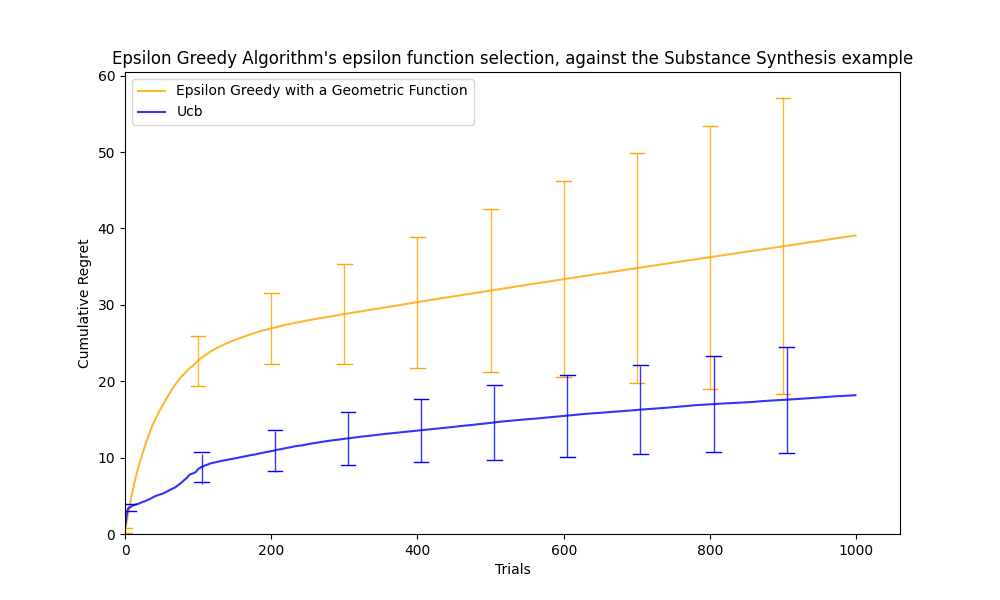
\includegraphics[width=17cm]{report/images/UCB-trumping-epsilon-greedy-SS.png}
    \caption{UCB performs very well on scenarios with not too many arms}
    \label{fig:ucb-ss}
\end{figure}

\begin{figure}[h!]
    \centering
    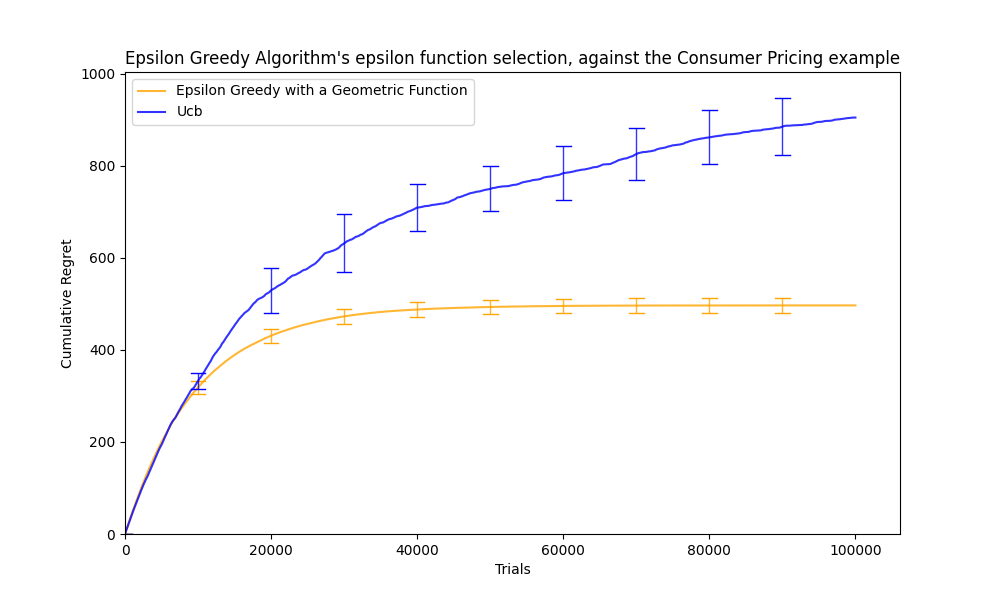
\includegraphics[width=17cm]{report/images/UCB-worse-over-ages-cp.png}
    \caption{UCB performs poorly when there are too many arms}
    \label{fig:ucb-cp}
\end{figure}

\subsubsection{It's not flexible}

When we have prior data, using the Epsilon-Greedy algorithm allows us to estimate or choose an \(\epsilon\) value that could potentially reduce regret, even if only slightly. However, UCB has no mechanism at all in incorporating prior information about a bandit scenario, making it a poor choice in these scenarios.

\subsection{Thompson Sampling (BernTS)}

The Thompson sampling algorithm also has no time-complexity problems when implemented, since it's only $\bigO{K}$.

Due to its balance between randomness and logical consistency by sampling beta distributions, the selection strategies it produces vary to some extent. This variability is absent in other algorithms, like UCB, which can make them behave predictably when presented with certain arm values, leading to sub-optimal behaviour and increased regret. BernTS, with its randomized sampling approach, sidesteps these "trap" scenarios by employing a non-deterministic selection strategy.

What's more, even with very small priors for successes and failures for each arm, the algorithm's regret is reduced drastically with the correct implementation, such as Figure \label{fig:bernts-good-prior}.

\begin{figure}[h!]
    \centering
    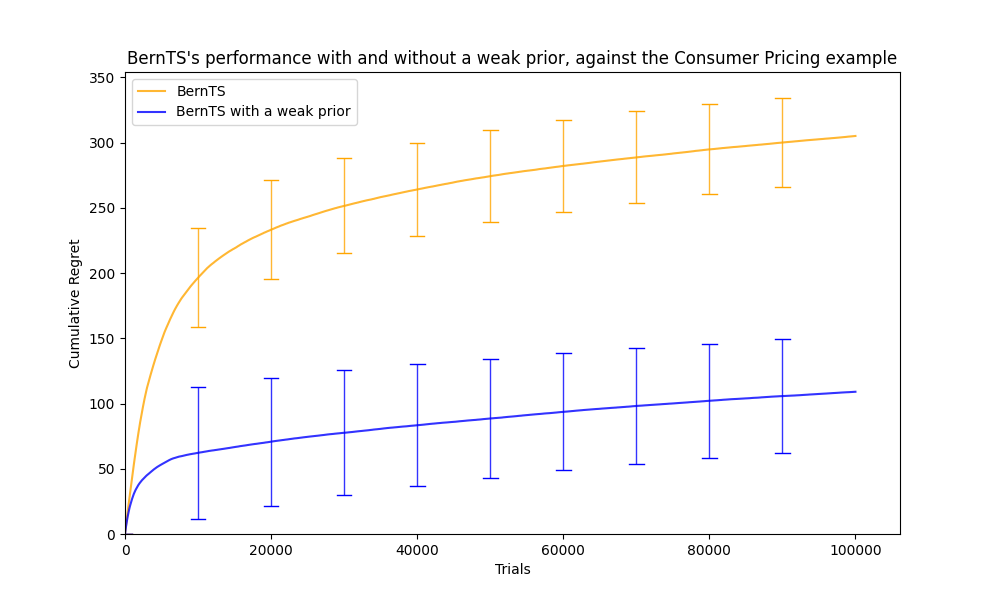
\includegraphics[width=17cm]{report/images/BernTS-good-priors-cp.png}
    \caption{The BernTS algorithm's regret when given weak prior information is reduced substantially}
    \label{fig:bernts-good-prior}
\end{figure}

\subsubsection{Priors are really sensitive}\label{sensitive_priors}

Although being able to incorporate prior information is very useful, it's important to consider how to translate this into BernTS's alpha and beta priors. The naïve approach to implement the prior information for Consumer Pricing (shown in Figure \ref{fig:bernts-bad-prior}) by simply setting alpha\_prior = [1, 3, 3, 3, 3, 1, 3, 3, 2, 3, 2, 2, 3, 2, 2, 2, 2, 2, 3, 3] appears sensible, however since all the arms have a very low success rate, this ends up throttling the learning rate substantially, as the prior has a much larger influence for longer. Since it's a very weak prior, and the results are not very accurate, this makes the slow learning rate increase cumulative regret much more than usual. A more sensible implementation is to dilute the alpha prior's strength by setting the beta prior of each arm to be 100 (which was done in Figure \ref{fig:bernts-good-prior}), simulating the additional known prior information that the arms likely have a low success rate.

\begin{figure}[h!]
    \centering
    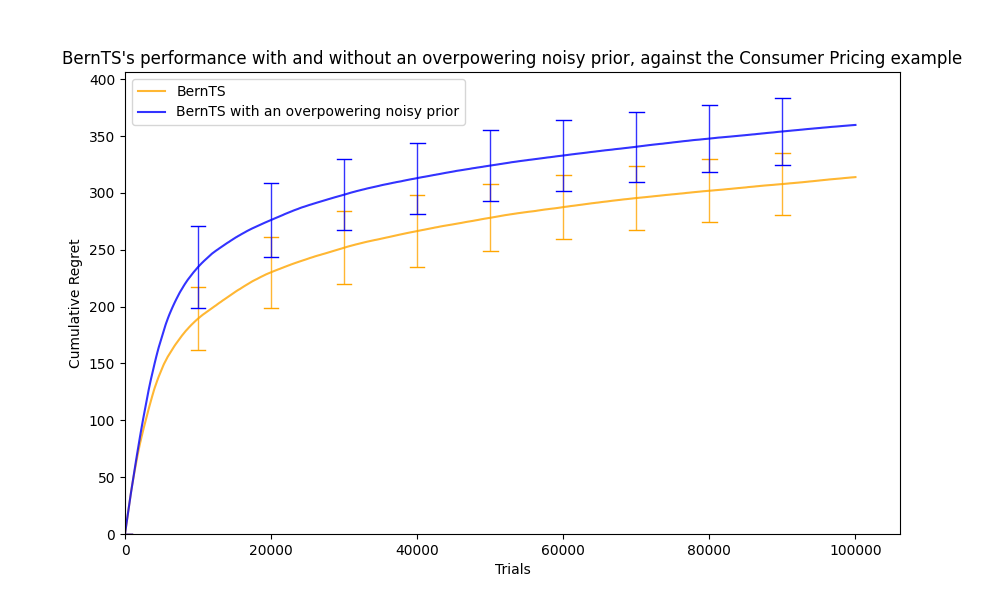
\includegraphics[width=17cm]{report/images/BernTS-bad-priors-cp.png}
    \caption{However, not interpreting prior information correctly can result in the BernTS algorithm's learning rate to suffer}
    \label{fig:bernts-bad-prior}
\end{figure}


\section{Pure Exploration Bandit Algorithms}

\subsection{Practicality of the Track and Stop Algorithm}

Unlike all of our classical bandit algorithms, the Track-and-Stop algorithm has several problems when we try to implement it via programming:

\subsubsection{Best arm notation}

It doesn't make any sense to assume that arm 1 is the best option for implementation purposes, as we lack a mathematical-proof oracle to designate which arm should be labeled as arm 1. Even if we did have this information, the algorithm would serve no purpose - it would simply recommend choosing arm 1.

Hence, we need some extra notation to define this. We already have:

$$\maxMeanArm(t) = \arg\max\limits_{k \in [K]}{\empiricalMeanReward{k}{t}}$$

$$\maxArmIndices(\mean) \coloneqq \arg\max\limits_{k \in [K]}{\armPopulationMean{k}}$$ 

To be the arm indices with the largest empirical and true mean. We also need a minimise equivalent, as we will see later. Hence, we can define, for a given $\mean$:

$$\minsub{f(i)} \coloneqq \min\{f(i) \mid i \in \mathbb{N}, i \not\in \maxArmIndices(\mean)\}
$$

\subsubsection{Taking the infimum}

We also have a problem with taking the infimum, since it's not practical to iterate over all possible alternative bandits within a reasonable timeframe. Hence, we can rearrage it as follows:

Given $\alpha = (\alpha_i)_{i=1}^k \in [0,1]^k$ such that $\sum_{i=1}^k\alpha_i=1$, we define
\begin{align*}
\Psi_{t}(\vectorBanditMeans, \alpha) &:=t\inf\limits_{\aDifBandit \in \banditSpace_{alt}(\vectorBanditMeans)}\left(\sum_{i=1}^{k} \alpha_i D(\vectorBanditMeans_{i}(t), \aDifBandit_{i})\right)\\
&=t\inf\limits_{\aDifBandit \in \banditSpace_{alt}(\vectorBanditMeans)}\left\lbrace \sum_{i=1}^{k}  \frac{\alpha_i\left(\armPopulationMeanSpecific{i}{\vectorBanditMeans(t)}- \armPopulationMeanSpecific{i}{\aDifBandit}\right)^2}{2\sigma_i^2}\right\rbrace.
\end{align*} 

In addition, we will $Z_t:=\Psi_{t}(\vectorBanditMeans, \hat{\alpha}(t))$ where $\hat{\alpha}(t) = (\hat{\alpha}_i(t))_{i=1}^k$ defined by $\hat{\alpha}_i(t)=\totalFunction{i}{t}/t$ so that

\begin{align*}
Z_t=\Psi_{t}(\vectorBanditMeans, \hat{\alpha}(t))
&= \inf\limits_{\aDifBandit \in \banditSpace_{alt}(\vectorBanditMeans)}\left\lbrace \sum_{i=1}^{k}  \totalFunction{i}{t} \cdot D(\vectorBanditMeans_{i}(t), \aDifBandit_{i})\right\rbrace 
\\&= t \cdot \inf\limits_{\aDifBandit \in \banditSpace_{alt}(\vectorBanditMeans)}\left\lbrace \sum_{i=1}^{k}  \hat{\alpha}_i(t) \cdot D(\vectorBanditMeans_{i}(t), \aDifBandit_{i})\right\rbrace 
\end{align*}

Using the method from this \cite{Lattimore_Szepesv´ar} paper, we can break down this infimum by noticing that minimised solutions "disturb" the empirical distributions least, since we are taking a modified cumulative relative entropy distance. Hence, in order to minimise the error, we should only sacrifice two error potentials - assuming the empirical mean of the best arm and some other non-optimal arm are the same. This way, the best arm is no longer uniquely optimal

More mathematically, this means all the relative entropy distances are zero, except the arm indices of our original and chosen arm. This lends itself to, assuming j is optimal and $\alpha_j = \hat{\alpha}_j(t)$, we can say $\xi_i = \{ \aDifBandit \in \xi \mid \armPopulationMeanSpecific{1}{\aDifBandit} = \armPopulationMeanSpecific{j}{\aDifBandit} , \space \armPopulationMeanSpecific{j}{\aDifBandit} = \armPopulationMeanSpecific{j}{\bandit} \space \forall j \not\in \{1, j\} \}$:

\begin{align*}
&= t \cdot \minsub \inf\limits_{\aDifBandit \in \xi_i}\left\lbrace \alpha_j D(\vectorBanditMeans_{j}(t), \aDifBandit_{j}) + \alpha_i D(\vectorBanditMeans_{i}(t), \aDifBandit_{i})\right\rbrace
\\&= t \cdot \minsub \inf\limits_{\aDifBandit \in \R}\left\lbrace \frac{\alpha_j\left(\armPopulationMeanSpecific{j}{\vectorBanditMeans(t)}- \armPopulationMeanSpecific{j}{\aDifBandit}\right)^2}{2\sigma_j^2} + \frac{\alpha_i\left(\armPopulationMeanSpecific{i}{\vectorBanditMeans(t)}- \armPopulationMeanSpecific{i}{\aDifBandit}\right)^2}{2\sigma_i^2}\right\rbrace
\\&= \frac{t}{2} \cdot \minsub \inf\limits_{\aDifBandit \in \R}\left\lbrace \frac{\alpha_j\left(\armPopulationMeanSpecific{j}{\vectorBanditMeans(t)}- \armPopulationMeanSpecific{j}{\aDifBandit}\right)^2}{\sigma_j^2} + \frac{\alpha_i\left(\armPopulationMeanSpecific{i}{\vectorBanditMeans(t)}- \armPopulationMeanSpecific{i}{\aDifBandit}\right)^2}{\sigma_i^2}\right\rbrace
\end{align*}

$$
Z_t = \frac{t}{2}\min_{i \not\in \maxArmIndices(\mean)}\frac{\alpha_1 \alpha_i \gap{i}^2}{\alpha_1 \sigma_i^2 + \alpha_i \sigma_1^2}.$$

Perhaps the simplest way will be to use this expression is to re-parameterise $\alpha$ as a vector $\beta_1,...,\beta_K \in \R $ via $ \alpha_i = e^{\beta_i}/(\sum_j e^{\beta_j})$. This way you don't need any additional constraints to encode probability vectors.

Let $\alpha_i = \frac{e^{\beta_i}}{c}$ with $c := \sum_j e^{\beta_j}$

Using that, $\sigma_i = 1 \forall i$:
$$Z_{t}(\vectorBanditMeans) = \frac{t}{2}\minsub\frac{\gap{i}^2}{c} \frac{e^{\beta_1} e^{\beta_i}}{e^{\beta_1} + e^{\beta_i}}
=\frac{t}{2c}\minsub   \frac{\Delta_i^2}{\sigma_i^2e^{-\beta_i} +\sigma_1^2 e^{-\beta_1} }$$

This is quite difficult to evaluate, since the minimisation may result in the values of $e^{-\beta_i}$ getting large enough such that the whole expression gets so small it rounds down to zero, which isn't very helpful. Therefore, we can take the log and minimise over it.

So, we can minimise:
\begin{align}
\log(Z_{t}(\vectorBanditMeans)) &=\log\left(\frac{t}{2c}\minsub   \frac{\Delta_i^2}{\sigma_i^2e^{-\beta_i} +\sigma_1^2 e^{-\beta_1} }\right) \\
&=\log\left(\frac{t}{2c}\right) + \log\left(\minsub \frac{\Delta_i^2}{\sigma_i^2e^{-\beta_i} +\sigma_1^2 e^{-\beta_1} }\right) \\
&=log\left(t\right)-\log\left(2\right) -\log\left(c\right) + \minsub \log\left(\frac{\Delta_i^2}{\sigma_i^2e^{-\beta_i} +\sigma_1^2 e^{-\beta_1} }\right) \\
\log(Z_{t}(\vectorBanditMeans))&=log\left(t\right)-\log\left(2\right) -\log\left(c\right) + \minsub \left(2\log\left(\Delta_i\right) -\log\left({\sigma_i^2e^{-\beta_i} +\sigma_1^2 e^{-\beta_1} }\right)\right)
\end{align}

